\part{Linear-Systems}
\lecture{Linear Systems}{Linear-Systems}
\section{Linear Systems}

\title{Ordinary Differential Equations}
\subtitle{Math 232 - Solutions to Linear Systems}
\date{26 Sep 2012}

\begin{frame}
  \titlepage
\end{frame}

\begin{frame}
  \frametitle{Outline}
  \tableofcontents[ currentsection ]
\end{frame}


\subsection{Linear Systems}


\begin{frame}
  \frametitle{What is a solution to a linear system?}

  \begin{eqnarray*}
    3x + y & = & 4 \\
    -2x + y & = & 2
  \end{eqnarray*}

  What is the value of $x$ and $y$?

  \only<2->{%

    Geometric Interpretation:

    \centerline{\includegraphics[width=4cm]{img/solvingTwoUnkowns}}

    }

\end{frame}


\begin{frame}
  \frametitle{What is a solution to a linear system?}

  \begin{eqnarray*}
    3x + y & = & 4 \\
    -2x + y & = & 2
  \end{eqnarray*}

  What is the value of $x$ and $y$?

  How can solve this analytically?
  \begin{itemize}
  \item Solve for $x$, substitute into the second equation, solve
    for $y$, and then substitute that result back in to the first
    equation.
  \item What if you have hundreds of equations and hundreds of
    unknowns?
  \item We need a better way!
  \end{itemize}

\end{frame}


\begin{frame}
  \frametitle{Canceling variables in a clever way}

  \begin{eqnarray*}
    3x + y & = & 4 \\
    -2x + y & = & 2 \\
    \\
    \Rightarrow
    x + \frac{1}{3}y & = & \frac{4}{3} \\
    -2x + y & = & 2 \\
  \end{eqnarray*}

  Now take 2*(Equation 1) + (Equation 2).

\end{frame}


\begin{frame}
  \frametitle{Canceling variables in a clever way}

  \begin{eqnarray*}
    x + \frac{1}{3}y & = & \frac{4}{3} \\
    \frac{5}{3}  y & = & \frac{14}{3} \\
  \end{eqnarray*}

  Solving for $y$ first we get
  \begin{eqnarray*}
    y & = & \frac{14}{5}.
  \end{eqnarray*}

  Now substitute back into the first equation to get
  \begin{eqnarray*}
    x & = & \frac{4}{3} - \frac{1}{3} y \\
    & = & \frac{2}{5}
  \end{eqnarray*}

  The two lines meet at the point $x=\frac{2}{5}$ and $y=\frac{14}{5}$.

\end{frame}

\subsection{Solving in Matrix Notation}

\begin{frame}
  \frametitle{Using Matrix Notation}

  \begin{eqnarray*}
    \arrayTwo{3}{1}{-2}{1} \vecTwo{x}{y} & = & \vecTwo{4}{2} \\
    \uncover<1->{
      \Rightarrow
      \stateTwo{R_1/3}{~}
      \arrayTwo{1}{\frac{1}{3}}{-2}{1} \vecTwo{x}{y} & = & \vecTwo{\frac{4}{3}}{2} \\
    }
    \uncover<1->{
      \Rightarrow
      \stateTwo{~}{2R_1+R2}
      \arrayTwo{1}{\frac{1}{3}}{0}{\frac{5}{3}} \vecTwo{x}{y} & = & \vecTwo{\frac{4}{3}}{\frac{14}{3}}
    }
  \end{eqnarray*}
  \uncover<1->{Exactly the same thing only I am using matrices to
    track the coefficients.}

\end{frame}



\iftoggle{clicker}{%
\begin{frame}
  \frametitle{Clicker Quiz}

      \ifnum\value{clickerQuiz}=1{%

        \vfill

        Express the following system of equations in matrix/vector notation:
        \begin{eqnarray*}
          2x + 4y - z & = & 6 \\
          x + y + z & = & 2 \\
          -3x + y + 2z & = & 7
        \end{eqnarray*}

        \begin{eqnarray*}
          \begin{array}{l@{\hspace{2em}}rcl}
            A: & \arrayThree{2}{4}{-1}{1}{1}{1}{-3}{1}{2} \vecThree{x}{y}{z} & = & \vecThree{6}{2}{7}\\ [18pt]
            B: & \arrayThree{2}{1}{-3}{4}{1}{1}{-1}{1}{2} \vecThree{x}{y}{z} & = & \vecThree{6}{2}{7}\\
          \end{array}
        \end{eqnarray*}

          \vfill

     }\fi

     \ifnum\value{clickerQuiz}=2{%

        \vfill

        Express the following system of equations in matrix/vector notation:
        \begin{eqnarray*}
          2x + 4y - z & = & 6 \\
          x + y + z & = & 2 \\
          -3x + y + 2z & = & 7
        \end{eqnarray*}

        \begin{eqnarray*}
          \begin{array}{l@{\hspace{2em}}rcl}
            A: & \arrayThree{2}{4}{-1}{1}{1}{1}{-3}{1}{2} \vecThree{x}{y}{z} & = & \vecThree{6}{2}{7}\\ [18pt]
            B: & \arrayThree{2}{1}{-3}{4}{1}{1}{-1}{1}{2} \vecThree{x}{y}{z} & = & \vecThree{6}{2}{7}\\
          \end{array}
        \end{eqnarray*}

          \vfill


     }\fi

      \ifnum\value{clickerQuiz}=3{%

        \vfill

        Express the following system of equations in matrix/vector notation:
        \begin{eqnarray*}
          2x + 4y - z & = & 6 \\
          x + y + z & = & 2 \\
          -3x + y + 2z & = & 7
        \end{eqnarray*}

        \begin{eqnarray*}
          \begin{array}{l@{\hspace{2em}}rcl}
            A: & \arrayThree{2}{4}{-1}{1}{1}{1}{-3}{1}{2} \vecThree{x}{y}{z} & = & \vecThree{6}{2}{7}\\ [18pt]
            B: & \arrayThree{2}{1}{-3}{4}{1}{1}{-1}{1}{2} \vecThree{x}{y}{z} & = & \vecThree{6}{2}{7}\\
          \end{array}
        \end{eqnarray*}

          \vfill


     }\fi

    \vfill
    \vfill
    \vfill

\end{frame}

}





\begin{frame}

  \begin{eqnarray*}
    \stateThree{R_1/2}{~}{~}
    \arrayThree{1}{2}{-0.5}{1}{1}{1}{-3}{1}{2} \vecThree{x}{y}{z} & = & \vecThree{3}{2}{7} \\
    \uncover<1->
    {
      \stateThree{~}{-R_1+R_2}{3R_1+R_3}
      \arrayThree{1}{2}{-0.5}{0}{-1}{1.5}{0}{7}{0.5} \vecThree{x}{y}{z} & = & \vecThree{3}{-1}{16} \\
    }
    \uncover<1->
    {
      \stateThree{~}{-R_2}{~}
      \arrayThree{1}{2}{-0.5}{0}{1}{-1.5}{0}{7}{0.5} \vecThree{x}{y}{z} & = & \vecThree{3}{1}{16} \\
    }
    \uncover<1->
    {
      \stateThree{~}{~}{-7R_2+R_3}
      \arrayThree{1}{2}{-0.5}{0}{1}{-1.5}{0}{0}{11} \vecThree{x}{y}{z} & = & \vecThree{3}{1}{9}
    }
  \end{eqnarray*}

\end{frame}


\begin{frame}
  \frametitle{Note}

  \begin{eqnarray*}
    \stateThree{~}{~}{R_3/11}
    \arrayThree{1}{2}{-0.5}{0}{1}{-1.5}{0}{0}{1} \vecThree{x}{y}{z} & = & \vecThree{3}{1}{9/11} \\
    \uncover<1->
    {
      \stateThree{R_1+ 1/2 R_3}{R_2 + 3/2 R_3}{~}
      \arrayThree{1}{2}{0}{0}{1}{0}{0}{0}{1} \vecThree{x}{y}{z} & = & \vecThree{75/22}{49/22}{9/11} \\
    }
    \uncover<1->
    {
      \stateThree{R_1-2R_2}{~}{~}
      \arrayThree{1}{0}{0}{0}{1}{0}{0}{0}{1} \vecThree{x}{y}{z} & = & \vecThree{-23/22}{49/22}{9/11}
    }
  \end{eqnarray*}
  \uncover<1->{``Reduced Row Echelon'' See definition at the top of page 136.}

\end{frame}

\subsection{More Compact Notation}

\begin{frame}
  \frametitle{Example}

  \begin{eqnarray*}
    2x + 4y + 6z & = & 8 \\
    x - y + z & = & 4 \\
    4x + 2y + 8z & = & 4 \\
    ~ \\
    \uncover<1->
    {
      \stateThree{~}{~}{~}
      \startRowOps
      \oneRowOps{2}{4}{6}{8}
      \oneRowOps{1}{-1}{1}{4}
      \oneRowOps{4}{2}{8}{4}
      \stopRowOps
    }
    \\
    \uncover<1->
    {
      \stateThree{R_1/2}{~}{~}
      \startRowOps
      \oneRowOps{1}{2}{3}{4}
      \oneRowOps{1}{-1}{1}{4}
      \oneRowOps{4}{2}{8}{4}
      \stopRowOps
    }
  \end{eqnarray*}

\end{frame}


\begin{frame}
  \frametitle{Example}

  \begin{eqnarray*}
      \stateThree{~}{-R_1+R_2}{-4R_1+R_3}
      \startRowOps
      \oneRowOps{1}{2}{3}{4}
      \oneRowOps{0}{-3}{-2}{0}
      \oneRowOps{0}{-6}{-4}{-12}
      \stopRowOps    \\
      \uncover<1->
      {
        \stateThree{~}{-1/3 R_2}{~}
        \startRowOps
        \oneRowOps{1}{2}{3}{4}
        \oneRowOps{0}{1}{2/3}{0}
        \oneRowOps{0}{-6}{-4}{-12}
        \stopRowOps    \\
      }
      \uncover<1->
      {
        \stateThree{~}{~}{6R_2+R_3}
        \startRowOps
        \oneRowOps{1}{2}{3}{4}
        \oneRowOps{0}{1}{2/3}{0}
        \oneRowOps{0}{0}{0}{-12}
        \stopRowOps
      }
  \end{eqnarray*}

  \uncover<1-> { If one row comes out with zeros except in the last
    column we say that the system is ``not consistent.''}

\end{frame}


\begin{frame}
  \frametitle{Example}
  Suppose instead the system looks like the following:

  \begin{eqnarray*}
    2x + 4y + 6x & = & 8 \\
    x - y + z & = & 4 \\
    4x + 2y + 8z & = & 16 \\
    ~ \\
    \uncover<1->
    {
      \stateThree{~}{~}{~}
      \startRowOps
      \oneRowOps{2}{4}{6}{8}
      \oneRowOps{1}{-1}{1}{4}
      \oneRowOps{4}{2}{8}{16}
      \stopRowOps
    }
    \\
    \uncover<1->
    {
      \stateThree{~}{~}{~}
      \startRowOps
      \oneRowOps{1}{2}{3}{4}
      \oneRowOps{0}{1}{2/3}{0}
      \oneRowOps{0}{0}{0}{0}
      \stopRowOps
    }
  \end{eqnarray*}


  \uncover<1->{If you get all zeros across all of the columns of one
    row so that you have less than ``n'' non-zero rows then the system
    is called ``underdetermined.''}

\end{frame}

\begin{frame}
  \frametitle{The RREF of the previous example}

  The RREF of the previous system is the following:
  \begin{eqnarray*}
    \stateThree{~}{~}{~}
    \startRowOps
    \oneRowOps{1}{0}{5/3}{4}
    \oneRowOps{0}{1}{2/3}{0}
    \oneRowOps{0}{0}{0}{0}
    \stopRowOps
  \end{eqnarray*}

  What does it mean?

  \begin{eqnarray*}
    y + \frac{2}{3}z & = & 0, \\
    \Rightarrow y & = & -\frac{2}{3} z
  \end{eqnarray*}

  \uncover<1->
  {
    \begin{eqnarray*}
      x + \frac{5}{3} z & = & 4, \\
      \Rightarrow x & = & 4 - \frac{5}{3} z
    \end{eqnarray*}
  }

\end{frame}

\begin{frame}
  \frametitle{The Solution}

  \begin{eqnarray*}
    \vecThree{x}{y}{z} & = & \vecThree{4 - \frac{5}{3}z}{-\frac{2}{3}z}{z} \\
    & = & \vecThree{4}{0}{0} + z \vecThree{\frac{-5}{3}}{\frac{-2}{3}}{1}
  \end{eqnarray*}

  For any $z$!

\end{frame}

\iftoggle{clicker}{%
\begin{frame}
  \frametitle{Clicker Quiz}

      \ifnum\value{clickerQuiz}=1{%

        \vfill

        \begin{eqnarray*}
          \vecThree{x}{y}{z} & = & \vecThree{4 - \frac{5}{3}z}{-\frac{2}{3}z}{z} \\
          & = & \vecThree{4}{0}{0} + z \vecThree{\frac{-5}{3}}{\frac{-2}{3}}{1}
        \end{eqnarray*}

        How many solutions are there to the system?

        \begin{tabular}{{l@{\hspace{3em}}l}}
          A: & Infinite \\
          B: & One \\
          C: & None
        \end{tabular}


        \vfill

     }\fi

     \ifnum\value{clickerQuiz}=2{%

        \vfill

        \begin{eqnarray*}
          \vecThree{x}{y}{z} & = & \vecThree{4 - \frac{5}{3}z}{-\frac{2}{3}z}{z} \\
          & = & \vecThree{4}{0}{0} + z \vecThree{\frac{-5}{3}}{\frac{-2}{3}}{1}
        \end{eqnarray*}

        How many solutions are there to the system?

        \begin{tabular}{{l@{\hspace{3em}}l}}
          A: & None \\
          B: & One \\
          C: & Infinite
        \end{tabular}


        \vfill


     }\fi

      \ifnum\value{clickerQuiz}=3{%

        \vfill

        \begin{eqnarray*}
          \vecThree{x}{y}{z} & = & \vecThree{4 - \frac{5}{3}z}{-\frac{2}{3}z}{z} \\
          & = & \vecThree{4}{0}{0} + z \vecThree{\frac{-5}{3}}{\frac{-2}{3}}{1}
        \end{eqnarray*}

        How many solutions are there to the system?

        \begin{tabular}{{l@{\hspace{3em}}l}}
          A: & Infinite \\
          B: & One \\
          C: & None
        \end{tabular}



        \vfill


     }\fi

    \vfill
    \vfill
    \vfill

\end{frame}

}



\begin{frame}
  \frametitle{Another Way to Express The Solution}

  \begin{eqnarray*}
    \arrayThree{2}{4}{6}{1}{-1}{1}{4}{2}{8} \vecThree{-5/3}{-2/3}{1}
    & = & \vecThree{0}{0}{0}
  \end{eqnarray*}

  The homogeneous solution is
  \begin{eqnarray*}
    \vec{x}_h & = & \vecThree{-5/3}{-2/3}{1}.
  \end{eqnarray*}

\end{frame}

\begin{frame}
  \frametitle{Another Way to Express The Solution}

  \begin{eqnarray*}
    \arrayThree{2}{4}{6}{1}{-1}{1}{4}{2}{8} \vecThree{4}{0}{0}
    & = & \vecThree{8}{4}{16}
  \end{eqnarray*}

  The particular solution is
  \begin{eqnarray*}
    \vec{x}_p & = & \vecThree{4}{0}{0}
  \end{eqnarray*}

  \uncover<1->{The solution is
    \begin{eqnarray*}
      \vec{x} & = & \vec{x}_p + C \vec{x}_h
    \end{eqnarray*}
    where $C$ can be any real number.
  }

\end{frame}

\subsection{Interpreting the RREF}

\begin{frame}
  \frametitle{The RREF provides a lot of information}

  Suppose that we have
  \begin{eqnarray*}
    A\vec{x} & = & \vec{b}, \\
    \vec{x} & = &
    \left[ \begin{array}{r}x_1\\x_2\\x_3\\x_4\\x_5\end{array}\right]
  \end{eqnarray*}
  and the REF of the system is the following:
  \begin{eqnarray*}
    \left[
      \begin{array}{rrrrr|r}
        1 & 0 & 2 & 0 & 0 & 2 \\
        0 & 1 & -1 & 0 & 1 & 1 \\
        0 & 0 & 0 & 0 & 0 & 0 \\
        0 & 0 & 0 & 1 & 2 & 3 \\
        0 & 0 & 0 & 0 & 0 & 0
      \end{array}
    \right]
  \end{eqnarray*}

\end{frame}


\begin{frame}
  \frametitle{We can find solutions}


  \begin{eqnarray*}
    x_1 + 2x_3 & = & 2 \\
    x_2 - x_3 + x_5 & = & 1 \\
    x_4 + 2x_5 & = & 3
  \end{eqnarray*}
  or
  \begin{eqnarray*}
    x_1  & = & 2 -  2x_3\\
    x_2  & = & 1 +  x_3 - x_5\\
    x_4  & = & 3 - 2x_5
  \end{eqnarray*}

\end{frame}

\begin{frame}
  \frametitle{We can find solutions}

  In vector form:
  \begin{eqnarray*}
    \left[ \begin{array}{r}x_1\\x_2\\x_3\\x_4\\x_5\end{array}\right] & = &
    \left[ \begin{array}{r}2-2x_3\\1+x_3-x_5\\x_3\\3-2x_5\\x_5\end{array}\right]=
    \left[ \begin{array}{r}2-2x_3+0x_5\\1+1x_3-1x_5\\0+1x_3+0x_5\\3+0x_3-2x_5\\0+0x_3+1x_5\end{array}\right]
    \\
    & = &
    \left[ \begin{array}{r}2\\1\\0\\3\\0\end{array}\right]
    + x_3 \left[ \begin{array}{r}-2\\1\\1\\0\\0\end{array}\right]
    + x_5 \left[ \begin{array}{r}0\\-1\\0\\-2\\1\end{array}\right]
  \end{eqnarray*}

  where $x_3$ and $x_5$ can be any number.


\end{frame}


% LocalWords:  Clarkson pausesection hideothersubsections RREF
